\documentclass[a4paper]{article}

\usepackage[a4paper,  margin=0.4in]{geometry}
% \usepackage[left=2.5cm,top=3cm,right=2.5cm,bottom=3cm,bindingoffset=0.5cm]{geometry}

\usepackage{graphicx}
\usepackage{float}
\usepackage{hyperref}
\usepackage{multicol}


\usepackage[utf8]{inputenc}
\begin{document}

% \begin{titlepage}
\title{SNR classes project - birds species recognition using deep neural networks
- second stage report}

\author{Michał Sypetkowski, Marcin Lew}
\twocolumn
\maketitle


\section{General information}
Git repository:\newline
\url{https://github.com/msypetkowski/SNR-proj.git}.\newline
Previous stage report: \newline
\url{https://github.com/msypetkowski/SNR-proj/blob/master/doc/main.pdf}.

In all experiments we use Adam optimizer and we exponentially
decrease learning rate by 50\% for 1000 iterations.
We use batch size of 128.

The whole document is a sequence of sections corresponding to various experiments. 
Accuracy curves for the model for current experiment and for the best model from previous experiments,
are always shown in a graph.
(the exception is section \ref{expLayer} where only current results are shown, because there was no preceding experiments).

\section{Establishing Layers count}
\label{expLayer}

First, we experimented with layers count.
    We trained 3 different models (they have 11, 8 and 6 layers respectively).
Detailed layers descriptions for each model are shown in tables
\ref{table:layers11},
\ref{table:layers8} and
\ref{table:layers6} respectively.
Rounded total trainable parameters count is respectively: 2.0M, 1.7M  and 1.5M.

Batch normalization with relu activation layers are used in all these models,
where the horizontal lines occur in the tables.

\begin{table}[!h]
    \caption{11-convolutional-layers convolutional NN architecture.
    \label{table:layers11}
    }
\begin{center}
    \begin{tabular}{| l | l | l | l |}
    \hline
        Layer & kernel/window& strides & output shape\\
    \hline
        Conv1  & (5, 5)&        (1, 1)&     224x224x64  \\
    \hline
        MaxPool1 & (2, 2)&      (2, 2)&     112x112x64  \\
        Conv2  & (5, 5)&        (1, 1)&     112x112x64  \\
    \hline
        MaxPool2 & (2, 2)&      (2, 2)&     56x56x64    \\
        Conv3  & (5, 5)&        (1, 1)&     56x56x64    \\
    \hline
        MaxPool3 & (2, 2)&      (2, 2)&     28x28x64    \\
        Conv4  & (5, 5)&        (1, 1)&     28x28x64  \\
    \hline
        MaxPool4 & (2, 2)&      (2, 2)&     14x14x64  \\
        Conv5  & (5, 5)&        (1, 1)&     14x14x64  \\ % additional
    \hline
        MaxPool5 & (2, 2)&      (1, 1)&     14x14x64  \\
        Conv6  & (5, 5)&        (1, 1)&     14x14x64  \\
    \hline
        MaxPool6 & (2, 2)&      (2, 2)&     7x7x64  \\
        Conv7  & (5, 5)&        (1, 1)&     7x7x64  \\  % additional
    \hline
        MaxPool7 & (2, 2)&      (1, 1)&     7x7x64  \\
        Conv8  & (3, 3)&        (1, 1)&     7x7x128\\
    \hline
        MaxPool8 & (2, 2)&      (2, 2)&     4x4x128  \\
        Conv9  & (2, 2)&        (1, 1)&     4x4x128)\\
    \hline
        MaxPool9 & (2, 2)&      (1, 1)&     4x4x128  \\
        Conv10 & (2, 2)&        (1, 1)&     4x4x128)\\  % additional
    \hline
        MaxPool10 & (2, 2)&      (1, 1)&     4x4x128  \\
        Conv11 & (3, 2)&        (1, 1)&     4x4x128)\\  % 4x4
    \hline
        MaxPool11 & (2, 2)&      (1, 1)&     4x4x128  \\
        Flatten & - & - & 2048 \\
        Dense1 & - & - & 512 \\
    \hline
        Output & - & - & 50 \\
        Softmax & - & - & 50 \\
    \hline
    \end{tabular}
\end{center}
\end{table}

\begin{table}[!h]
    \caption{ 8-convolutional-layers convolutional NN architecture (layers names correspond to some layers names in 11-convolutional-layers architecture \ref{table:layers11}).
    \label{table:layers8}
    }
\begin{center}
    \begin{tabular}{| l | l | l | l |}
    \hline
        Layer & kernel/window& strides & output shape\\
    \hline
        Conv1  & (5, 5)&        (1, 1)&     224x224x64  \\
    \hline
        MaxPool1 & (2, 2)&      (2, 2)&     112x112x64  \\
        Conv2  & (5, 5)&        (1, 1)&     112x112x64  \\
    \hline
        MaxPool2 & (2, 2)&      (2, 2)&     56x56x64    \\
        Conv3  & (5, 5)&        (1, 1)&     56x56x64    \\
    \hline
        MaxPool3 & (2, 2)&      (2, 2)&     28x28x64    \\
        Conv4  & (5, 5)&        (1, 1)&     28x28x64  \\
    \hline
        MaxPool4 & (2, 2)&      (2, 2)&     14x14x64  \\
        Conv6  & (5, 5)&        (1, 1)&     14x14x64  \\
    \hline
        MaxPool6 & (2, 2)&      (2, 2)&     7x7x64  \\
        Conv8  & (3, 3)&        (1, 1)&     7x7x128\\
    \hline
        MaxPool8 & (2, 2)&      (2, 2)&     4x4x128  \\
        Conv9  & (2, 2)&        (1, 1)&     4x4x128)\\
    \hline
        MaxPool9 & (2, 2)&      (1, 1)&     4x4x128  \\
        Conv11 & (3, 2)&        (1, 1)&     4x4x128)\\  % 4x4
    \hline
        MaxPool11 & (2, 2)&      (1, 1)&     4x4x128  \\
        Flatten & - & - & 2048 \\
        Dense1 & - & - & 512 \\
    \hline
        Output & - & - & 50 \\
        Softmax & - & - & 50 \\
    \hline
    \end{tabular}
\end{center}
\end{table}



\begin{table}[!h]
    \caption{6-convolutional-layers convolutional NN architecture (layers names correspond to some layers names in 11-convolutional-layers architecture \ref{table:layers11}).
    \label{table:layers6}
    }
\begin{center}
    \begin{tabular}{| l | l | l | l |}
    \hline
        Layer & kernel/window& strides & output shape\\
    \hline
        Conv1  & (5, 5)&        (1, 1)&     224x224x64  \\
    \hline
        MaxPool1 & (2, 2)&      (2, 2)&     112x112x64  \\
        Conv2  & (5, 5)&        (1, 1)&     112x112x64  \\
    \hline
        MaxPool2 & (2, 2)&      (2, 2)&     56x56x64    \\
        Conv3  & (5, 5)&        (1, 1)&     56x56x64    \\
    \hline
        MaxPool3 & (4, 4)&      (4, 4)&     28x28x64    \\
        Conv6  & (5, 5)&        (1, 1)&     14x14x64  \\
    \hline
        MaxPool6 & (2, 2)&      (2, 2)&     7x7x64  \\
        Conv8  & (3, 3)&        (1, 1)&     7x7x128\\
    \hline
        MaxPool8 & (2, 2)&      (2, 2)&     4x4x128  \\
        Conv11 & (3, 2)&        (1, 1)&     4x4x128)\\  % 4x4
    \hline
        MaxPool11 & (2, 2)&      (1, 1)&     4x4x128  \\
        Flatten & - & - & 2048 \\
        Dense1 & - & - & 512 \\
    \hline
        Output & - & - & 50 \\
        Softmax & - & - & 50 \\
    \hline
    \end{tabular}
\end{center}
\end{table}

\subsection{Results}
We used cross entropy as a loss function.
We trained each model for 5K iterations with initial learning rate of 0.03.
Accuracy curves are shown in figure \ref{fig:layersAcc}.

Training accuracy increases faster for models with fewer layers.
Smaller networks naturally learn faster, but they have fewer degrees of freedom
and may get worse results in the end.
11-convolutional-layers network architecture shown to be too complicated for
our dataset and/or training method.
Best accuracy was achieved by medium -- 8-convolutional-layers network.
We used this architecture for further experiments.

\begin{figure}[!h]
    \centering
    \includegraphics[page=2,width=0.5\textwidth]{curvesLayers.png}
    \caption[]{Accuracy curves for models with different layers count.
    \label{fig:layersAcc}
   	}
\end{figure}

\section{Experiments with size of the last convolutional layer}

Our 8-layer network from section \ref{expLayer}, outputs
feature vectors of size 2048 from the last convolutional layer (after flattening, see Conv11 in table \ref{table:layers8}).
We tried models with 1024 and 4096 sizes of these vectors.
The results are shown in figure \ref{fig:lastSize}.
These dimensions significantly affect total trainable parameters count
(around 1.1M in case of 1024 dimensions and around 2.8M in case of 4096 dimensions).

Decreasing or increasing this parameter caused only loss in accuracy
(models had in the end not enough or too many parameters for our dataset).
% 1024 1138674
% 4096 2810226

\begin{figure}[!h]
    \centering
    \includegraphics[page=2,width=0.5\textwidth]{lastConvSize.png}
    \caption[]{Accuracy curves for models with different last convolutional layer size.
    \label{fig:lastSize}
    }
\end{figure}


\section{Experiments with activation function}

We tested sigmoid activation function using 8-convolutional-layers network from section \ref{expLayer}.
We trained the sigmoid model variant for 5000 iterations longer.

As we can see in figure \ref{fig:sigmoid}, experimental model learns significantly slower,
but achieves only slightly worse result in the end.

Training accuracy grows relatively fast -- test accuracy
starts giving better answers than random choice (above 2\%),
when the training accuracy is above 90\%.
Experimental model learns more memory-like rules for first 3k iterations.
When this strategy achieves its limit, the generic rules emerge.
In the end, validation accuracy has sigmoid-like shape.



\begin{figure}[!h]
    \centering
    \includegraphics[page=2,width=0.5\textwidth]{sigmoidConv.png}
    \caption[]{Accuracy curves for model with sigmoid activation function.
    \label{fig:sigmoid}
    }
\end{figure}


\section{Experiments with loss function}

We tested MSE (Mean Squared Error) as activation function instead of cross entropy.
Nowadays, it is a common knowledge that using cross entropy in classification models works much better than instead of
MSE.

In our experiment, MSE works generally worse during the whole training. Accuracy and training curves are shown in figure \ref{fig:mse}.

\begin{figure}[!h]
    \centering
    \includegraphics[page=2,width=0.5\textwidth]{sqrLoss.png}
    \caption[]{Accuracy curves for model with MSE loss function.
    \label{fig:mse}
    }
\end{figure}

\section{Experiments with SVMs}
\label{svm}

We experimented with using features from batch normalization layer after last dense layer and last convolutional layer (to be exact -- from flattening layer).
For training each SVM, we used 20k feature vectors.
We used various kernels in this experiment.
Last dense layer had 512 output features and last convolutional layer had 2048.
Results of this experiments are shown in table \ref{table:svm}.

Most surprising fact is that linear kernel after last convolutional gives
better results than variant without SVM.
In cases, where we trained SVMs after last convolutional layers we
used in fact a model with significantly fewer parameters (we had around 0.7M instead of 1.7M).
Inspired by this observation we did experiment described in section \ref{last}.

\begin{table}[!h]
    \caption{Accuracy for various SVMs usages.
    \label{table:svm}
    }
\begin{center}
    \begin{tabular}{| l | l | l | l |}
    \hline
    method&accuracy \\
    \hline
        noSVM & 46.3\% \\
        RBF after last dense & 49.3\% \\
        RBF after last convolutional & 49.6\% \\
        linear after last dense & 47.6\% \\
        linear after last convolutional & 48.0\% \\
        polynomial (degree=3) after last dense & 49.6\% \\
        polynomial (degree=3) after last convolutional & 51.3\% \\
        sigmoid after last dense & 46.0\% \\
        sigmoid after last convolutional & 37.0\% \\
    \hline
    \end{tabular}
\end{center}
\end{table}

\section{Experiment with removing dense layer}
\label{last}

Inspired by results achieved in previous section,
we trained model without last dense layer.
New model had 0.7M trainable parameters instead of 1.7M.
Accuracy curves are shown in figure \ref{fig:noDense},
and SVM experiments results -- in table \ref{table:svm2}.

As we can see, training SVMs after flattened last convolutional
layer output gives only worse results in this case.

This experiment showed that sometimes training model with a certain
amount of trainable parameters, then removing more than a half
of them (in our case decreasing from 1.7M to 0.7M) and adding SVM,
may actually give better results than training model with lower
parameters count from the beginning and then adding SVM.

\begin{figure}[!h]
    \centering
    \includegraphics[page=2,width=0.5\textwidth]{noDense.png}
    \caption[]{Accuracy curves for 8-convolutional-convolutional-layers model without dense layer.
    \label{fig:noDense}
    }
\end{figure}

\begin{table}[!hbt]
    \caption{Accuracy for various SVMs usages (on model without last dense layer).
    \label{table:svm2}
    }
\begin{center}
    \begin{tabular}{| l | l | l | l |}
    \hline
    method&accuracy \\
    \hline
        noSVM & 40.0\% \\
        RBF after last convolutional & 39.6\% \\
        polynomial (degree=3) after last convolutional & 6\% \\
    \hline
    \end{tabular}
\end{center}
\end{table}

\section{Summary}
In this stage we did six experiments. Each experiment concerns
a particular element of neural network architecture.
In the end, best accuracy is achieved by model with:
\begin{itemize}
    \item 8 convolutional layers
    \item relu activation function
    \item cross entropy loss function
    \item SVM with polynomial kernel (degree=3) after last convolutional layer
\end{itemize}

\end{document}
